\begin{table}[H]\centering
\caption{Model configurations}\label{tab:S1}
\small
\begin{tabular}{>{\raggedright\arraybackslash}p{0.367647\dimexpr\textwidth-14\tabcolsep\relax}>{\raggedright\arraybackslash}p{0.073529\dimexpr\textwidth-14\tabcolsep\relax}>{\raggedright\arraybackslash}p{0.088235\dimexpr\textwidth-14\tabcolsep\relax}>{\raggedright\arraybackslash}p{0.117647\dimexpr\textwidth-14\tabcolsep\relax}>{\raggedright\arraybackslash}p{0.088235\dimexpr\textwidth-14\tabcolsep\relax}>{\raggedright\arraybackslash}p{0.117647\dimexpr\textwidth-14\tabcolsep\relax}>{\raggedright\arraybackslash}p{0.147059\dimexpr\textwidth-14\tabcolsep\relax}}
\toprule
\textbf{Model} & \textbf{Seed} & \textbf{Epochs} & \textbf{LR} & \textbf{Batch} & \textbf{Patches} & \textbf{Best epoch} \\
\midrule
Three-model ensemble & 42 & N/A & N/A & N/A & 512 & N/A \\
Hybrid-Evidence MIL & 42 & 30 & 5e-05 & 8 & 512 & 15 \\
ABMIL & 42 & 50 & 5e-05 & 16 & 512 & 37 \\
DTFD-style & 42 & 20 & 5e-05 & 8 & 512 & 11 \\
CLAM-SB-style & 42 & 20 & 5e-05 & 8 & 512 & 16 \\
RRTMIL-style & 42 & 20 & 5e-05 & 4 & 512 & 11 \\
ProtoMIL-style & 42 & 20 & 5e-05 & 8 & 512 & 14 \\
Mean pooling & 42 & 50 & 5e-05 & 16 & 512 & 35 \\
TransMIL-style & 42 & 20 & 5e-05 & 4 & 512 & 14 \\
DSMIL-style & 42 & 20 & 5e-05 & 8 & 512 & 17 \\
Distribution-ProtoMIL & 42 & 20 & 5e-05 & 8 & 512 & 8 \\
CONCH v1.5 + TITAN & 42 & 50 & 5e-05 & 1 & 1024 & 44 \\
\bottomrule
\end{tabular}

\par\medskip\footnotesize All rows refer to the internal MALT/SS task. The ensemble has no separate training epochs.
\end{table}

\begingroup\footnotesize
\renewcommand{\arraystretch}{1.12}
\begin{longtable}{@{}p{.29\textwidth}p{.18\textwidth}p{.45\textwidth}@{}}
\caption{Complete internal interval estimates}\label{tab:S2}\\
\toprule Model & Metric & Estimate (95\% interval) \\ \midrule\endfirsthead
\toprule Model & Metric & Estimate (95\% interval) \\ \midrule\endhead
\midrule\multicolumn{3}{r}{Continued on the next page}\\\endfoot\bottomrule\endlastfoot

Three-model ensemble & AUROC & \textbf{0.9649} (0.9097--1.0000) \\*

 & AUPRC & \textbf{0.9576} (0.8930--1.0000) \\*

 & Accuracy & \underline{87.76\%} (75.76\%--94.27\%) \\*

 & Sensitivity & \underline{91.30\%} (73.20\%--97.58\%) \\*

 & Specificity & 84.62\% (66.47\%--93.85\%) \\*

 & PPV & 84.00\% (65.35\%--93.60\%) \\*

 & NPV & 91.67\% (74.15\%--97.68\%) \\*

 & F1 & 0.8750 (0.7777--0.9583) \\

\addlinespace

Hybrid-Evidence MIL & AUROC & \underline{0.9599} (0.9046--0.9967) \\*

 & AUPRC & \underline{0.9514} (0.8864--0.9965) \\*

 & Accuracy & \underline{87.76\%} (75.76\%--94.27\%) \\*

 & Sensitivity & \textbf{95.65\%} (79.01\%--99.23\%) \\*

 & Specificity & 80.77\% (62.12\%--91.49\%) \\*

 & PPV & 81.48\% (63.30\%--91.82\%) \\*

 & NPV & \underline{95.45\%} (78.20\%--99.19\%) \\*

 & F1 & \underline{0.8800} (0.7925--0.9583) \\

\addlinespace

ABMIL & AUROC & 0.9498 (0.8879--0.9933) \\*

 & AUPRC & 0.9396 (0.8675--0.9928) \\*

 & Accuracy & 85.71\% (73.33\%--92.90\%) \\*

 & Sensitivity & 82.61\% (62.86\%--93.02\%) \\*

 & Specificity & 88.46\% (71.02\%--96.00\%) \\*

 & PPV & 86.36\% (66.67\%--95.25\%) \\*

 & NPV & 85.19\% (67.52\%--94.08\%) \\*

 & F1 & 0.8444 (0.7273--0.9362) \\

\addlinespace

DTFD-style & AUROC & 0.9398 (0.8679--0.9916) \\*

 & AUPRC & 0.9416 (0.8786--0.9922) \\*

 & Accuracy & \underline{87.76\%} (75.76\%--94.27\%) \\*

 & Sensitivity & 86.96\% (67.87\%--95.46\%) \\*

 & Specificity & 88.46\% (71.02\%--96.00\%) \\*

 & PPV & 86.96\% (67.87\%--95.46\%) \\*

 & NPV & 88.46\% (71.02\%--96.00\%) \\*

 & F1 & 0.8696 (0.7619--0.9565) \\

\addlinespace

CLAM-SB-style & AUROC & 0.9365 (0.8612--0.9933) \\*

 & AUPRC & 0.9422 (0.8780--0.9930) \\*

 & Accuracy & \underline{87.76\%} (75.76\%--94.27\%) \\*

 & Sensitivity & \underline{91.30\%} (73.20\%--97.58\%) \\*

 & Specificity & 84.62\% (66.47\%--93.85\%) \\*

 & PPV & 84.00\% (65.35\%--93.60\%) \\*

 & NPV & 91.67\% (74.15\%--97.68\%) \\*

 & F1 & 0.8750 (0.7778--0.9583) \\

\addlinespace

RRTMIL-style & AUROC & 0.9281 (0.8328--0.9967) \\*

 & AUPRC & 0.8400 (0.7022--0.9964) \\*

 & Accuracy & \textbf{89.80\%} (78.24\%--95.56\%) \\*

 & Sensitivity & \textbf{95.65\%} (79.01\%--99.23\%) \\*

 & Specificity & 84.62\% (66.47\%--93.85\%) \\*

 & PPV & 84.62\% (66.47\%--93.85\%) \\*

 & NPV & \textbf{95.65\%} (79.01\%--99.23\%) \\*

 & F1 & \textbf{0.8980} (0.8163--0.9787) \\

\addlinespace

ProtoMIL-style & AUROC & 0.9264 (0.8411--0.9849) \\*

 & AUPRC & 0.9306 (0.8584--0.9862) \\*

 & Accuracy & 85.71\% (73.33\%--92.90\%) \\*

 & Sensitivity & 86.96\% (67.87\%--95.46\%) \\*

 & Specificity & 84.62\% (66.47\%--93.85\%) \\*

 & PPV & 83.33\% (64.15\%--93.32\%) \\*

 & NPV & 88.00\% (70.04\%--95.83\%) \\*

 & F1 & 0.8511 (0.7442--0.9362) \\

\addlinespace

Mean pooling & AUROC & 0.9247 (0.8411--0.9833) \\*

 & AUPRC & 0.9332 (0.8663--0.9851) \\*

 & Accuracy & 85.71\% (73.33\%--92.90\%) \\*

 & Sensitivity & 78.26\% (58.10\%--90.34\%) \\*

 & Specificity & \underline{92.31\%} (75.86\%--97.86\%) \\*

 & PPV & \underline{90.00\%} (69.90\%--97.21\%) \\*

 & NPV & 82.76\% (65.45\%--92.40\%) \\*

 & F1 & 0.8372 (0.7109--0.9362) \\

\addlinespace

TransMIL-style & AUROC & 0.9231 (0.8428--0.9900) \\*

 & AUPRC & 0.9180 (0.8295--0.9891) \\*

 & Accuracy & 81.63\% (68.64\%--90.02\%) \\*

 & Sensitivity & 65.22\% (44.89\%--81.19\%) \\*

 & Specificity & \textbf{96.15\%} (81.11\%--99.32\%) \\*

 & PPV & \textbf{93.75\%} (71.67\%--98.89\%) \\*

 & NPV & 75.76\% (58.98\%--87.17\%) \\*

 & F1 & 0.7692 (0.6061--0.9048) \\

\addlinespace

DSMIL-style & AUROC & 0.9197 (0.8378--0.9816) \\*

 & AUPRC & 0.9260 (0.8579--0.9825) \\*

 & Accuracy & 85.71\% (73.33\%--92.90\%) \\*

 & Sensitivity & 78.26\% (58.10\%--90.34\%) \\*

 & Specificity & \underline{92.31\%} (75.86\%--97.86\%) \\*

 & PPV & \underline{90.00\%} (69.90\%--97.21\%) \\*

 & NPV & 82.76\% (65.45\%--92.40\%) \\*

 & F1 & 0.8372 (0.7027--0.9333) \\

\addlinespace

Distribution-ProtoMIL & AUROC & 0.9130 (0.8227--0.9783) \\*

 & AUPRC & 0.9178 (0.8430--0.9789) \\*

 & Accuracy & 79.59\% (66.36\%--88.52\%) \\*

 & Sensitivity & \underline{91.30\%} (73.20\%--97.58\%) \\*

 & Specificity & 69.23\% (50.01\%--83.50\%) \\*

 & PPV & 72.41\% (54.28\%--85.30\%) \\*

 & NPV & 90.00\% (69.90\%--97.21\%) \\*

 & F1 & 0.8077 (0.7083--0.8980) \\

\addlinespace

CONCH v1.5 + TITAN & AUROC & 0.9013 (0.8026--0.9783) \\*

 & AUPRC & 0.9203 (0.8459--0.9798) \\*

 & Accuracy & 81.63\% (68.64\%--90.02\%) \\*

 & Sensitivity & \underline{91.30\%} (73.20\%--97.58\%) \\*

 & Specificity & 73.08\% (53.92\%--86.30\%) \\*

 & PPV & 75.00\% (56.64\%--87.32\%) \\*

 & NPV & 90.48\% (71.09\%--97.35\%) \\*

 & F1 & 0.8235 (0.7308--0.9167) \\

\addlinespace

\end{longtable}
\endgroup\normalsize

\clearpage

\begin{table}[H]\centering
\caption{Separate ensemble operating point}\label{tab:S3}
\small
\begin{tabular}{>{\raggedright\arraybackslash}p{0.285714\dimexpr\textwidth-4\tabcolsep\relax}>{\raggedright\arraybackslash}p{0.714286\dimexpr\textwidth-4\tabcolsep\relax}}
\toprule
\textbf{Metric} & \textbf{Estimate (95\% interval)} \\
\midrule
AUROC & 0.9649 (0.9097--1.0000) \\
Accuracy & 93.88\% (83.48\%--97.90\%) \\
Sensitivity & 91.30\% (73.20\%--97.58\%) \\
Specificity & 96.15\% (81.11\%--99.32\%) \\
F1 & 0.9333 (0.8511--1.0000) \\
\bottomrule
\end{tabular}

\par\medskip\footnotesize Threshold = 0.70; TN/FP/FN/TP = 25/1/2/21. This is an archived selected operating point.
\end{table}

\begin{table}[H]\centering
\caption{Paired internal model comparisons}\label{tab:S4}
\small
\begin{tabular}{>{\raggedright\arraybackslash}p{0.285714\dimexpr\textwidth-10\tabcolsep\relax}>{\raggedright\arraybackslash}p{0.142857\dimexpr\textwidth-10\tabcolsep\relax}>{\raggedright\arraybackslash}p{0.214286\dimexpr\textwidth-10\tabcolsep\relax}>{\raggedright\arraybackslash}p{0.200000\dimexpr\textwidth-10\tabcolsep\relax}>{\raggedright\arraybackslash}p{0.157143\dimexpr\textwidth-10\tabcolsep\relax}}
\toprule
\textbf{Comparison} & \textbf{AUROC difference} & \textbf{95\% interval} & \textbf{Discordant correct (Hybrid/other)} & \textbf{Exact McNemar P} \\
\midrule
Hybrid minus ABMIL & 0.0100 & -0.0184 to 0.0452 & 4/3 & 1.000 \\
Hybrid minus Three-model ensemble & -0.0050 & -0.0284 to 0.0167 & 1/1 & 1.000 \\
\bottomrule
\end{tabular}

\par\medskip\footnotesize Comparisons use the same 49 WSI and threshold 0.5. No multiplicity adjustment was applied. Intervals use 2,000 paired label-stratified bootstrap samples.
\end{table}

\begin{table}[H]\centering
\caption{External selected subgroups}\label{tab:S5}
\small
\begin{tabular}{>{\raggedright\arraybackslash}p{0.187500\dimexpr\textwidth-12\tabcolsep\relax}>{\raggedright\arraybackslash}p{0.312500\dimexpr\textwidth-12\tabcolsep\relax}>{\raggedright\arraybackslash}p{0.078125\dimexpr\textwidth-12\tabcolsep\relax}>{\raggedright\arraybackslash}p{0.078125\dimexpr\textwidth-12\tabcolsep\relax}>{\raggedright\arraybackslash}p{0.156250\dimexpr\textwidth-12\tabcolsep\relax}>{\raggedright\arraybackslash}p{0.187500\dimexpr\textwidth-12\tabcolsep\relax}}
\toprule
\textbf{Source} & \textbf{Archived stain tag} & \textbf{Label} & \textbf{WSI} & \textbf{Correct at 0.5} & \textbf{Median score} \\
\midrule
MALT\_BJ & H\&E-like & 1 & 33 & 23 & 0.8768 \\
MALT\_BJ & IHC / special stain & 1 & 111 & 111 & 0.8331 \\
MALT\_HE & HE archive & 1 & 8 & 8 & 0.9670 \\
SS\_BJ & SS (slide series) & 0 & 16 & 11 & 0.0543 \\
\bottomrule
\end{tabular}

\par\medskip\footnotesize The initial archive and the selected analysis are separate tables. Filename-derived case counts are not substituted for verified clinical patient counts.
\end{table}

\clearpage

\begin{table}[H]\centering
\caption{Linked performance and interpretation outputs}\label{tab:S6}
\small Individual-case rows are omitted from this public repository copy.
\end{table}

\begin{figure}[H]\centering
\fbox{\begin{minipage}[c][35mm][c]{.88\textwidth}\centering
\textbf{Omitted from this public repository copy}\\[6pt]
This figure contains tissue images or individual-slide observations.\\
The complete figure is retained in the local manuscript archive.
\end{minipage}}
\caption{\textbf{Internal diagnostic-group predictions and threshold behavior}. \textbf{a,} Individual Hybrid scores for the 23 MALT and 26 SS holdout slides. The dashed line marks 0.5. \textbf{b,} Sensitivity and specificity across thresholds for the same fixed predictions. Threshold variation does not represent an additional validation experiment.}\label{fig:S1}\end{figure}

\clearpage
\begin{table}[H]\centering
\caption{Acquisition parameters recovered from archived WSI metadata}\label{tab:S7}
\small
\begin{tabularx}{\textwidth}{@{}>{\raggedright\arraybackslash}Xrrr>{\raggedright\arraybackslash}p{.23\textwidth}@{}}
\toprule
Series & WSIs & Lens & MPP (x/y) & Recorded scanner \\
\midrule
Internal MALT/SS & 193 & $40\times$ & 0.225708 & Hamamatsu C9600-12 \\
External MALT: source B & 144 & $40\times$ & 0.225708 & Hamamatsu C9600-12 \\
External MALT: HE directory & 8 & $40\times$ & 0.225708 & Hamamatsu C9600-12 \\
External SS & 16 & $40\times$ & 0.225708 & Hamamatsu C9600-12 \\
\bottomrule
\end{tabularx}
\par\medskip\footnotesize MPP is in $\mu\mathrm{m}$ per level-0 pixel; the value is equal in both axes. TIFF headers recorded 44,305 pixels per centimetre. Internal files recorded NDP.scan 2.5.85 (133) or 3.3.0 (60); all 168 external files recorded 2.5.85. Coordinate attributes recorded target magnification $20\times$, patch size 512 pixels, level-0 footprint 1,024 pixels and zero overlap for all analyzed files. These metadata describe the archived images; clinical source and stain identities remain subject to provider confirmation.
\end{table}

\begin{table}[H]\centering
\caption{Supporting data and implementation files accompanying the draft}\label{tab:S8}
\small
\begin{tabularx}{\textwidth}{@{}>{\raggedright\arraybackslash}p{.21\textwidth}>{\raggedright\arraybackslash}X>{\raggedright\arraybackslash}p{.25\textwidth}@{}}
\toprule
Material & Contents & Access status \\
\midrule
Source Data draft archive & Publication-coded archived predictions; new same-bag external comparisons, 20-bag sampling outputs and internal-variable diagnostics; all nine controlled training runs, selected epochs and per-slide predictions; provisional reader aggregates; ROI contour and Brier analyses; recovered acquisition metadata. & Accompanies the local author-review draft; public release pending. \\
\addlinespace
Source Code draft archive & Archived custom MIL sources and configurations; new fixed-checkpoint inference and controlled-training runners, prespecified protocols, sampling schedules, dependency/runtime records, metric scripts and publication figure generators. & Accompanies the draft; public repository and licensing pending. \\
\addlinespace
Technical provenance record & Source/configuration/checkpoint and feature-file hashes; archived checkout identity; exact sampled-row indices; current execution metadata distinguished from the unrecovered historical training environment; acquisition and ROI provenance. & Included in the manuscript source package. \\
\addlinespace
Raw WSIs and clinical linkage & Original images, patient/case linkage, clinical characteristics and reference-diagnosis records. & Access arrangements require confirmation by the data-providing institutions. \\
\addlinespace
Individual reader decisions & Per-slide diagnoses, original scores and protocol records. & Held by the hospital data provider; pending incorporation into this draft. \\
\bottomrule
\end{tabularx}
\par\medskip\footnotesize Publication codes identify slides, not patients. The original-identifier mapping and blank clinical/reader confirmation forms are retained locally and excluded from the portable source package. No raw images or model weights are redistributed in these supporting archives.
\end{table}

\clearpage
\begin{table}[H]\centering
\caption{Input activation and gating in the configuration comparison}\label{tab:S9}
\small
\begin{tabularx}{\textwidth}{@{}>{\raggedright\arraybackslash}Xlllr@{}}
\toprule
Configuration & Active vectors & Statistics & Gate & AUROC \\
\midrule
Attention vector & A & Zeroed & Learned & 0.9281 \\
Attention + distribution & A, M, S & Zeroed & Learned & 0.9264 \\
+ high-margin vector + statistics & A, M, S, P & All eight & Learned & \underline{0.9482} \\
Full, equal gate & A, M, S, P, N & All eight & Equal & \textbf{0.9632} \\
Full, learned gate & A, M, S, P, N & All eight & Learned & \underline{0.9482} \\
\bottomrule
\end{tabularx}
\par\medskip\footnotesize Bold/underline denote the highest/second-highest displayed AUROC. A: attention; M: mean; S: standard deviation; P: high-margin vector; N: low-margin instance plus regional vector. Learned gates normalize over five positions, including masked vectors. All configurations retain the Hybrid fusion network. The transition to P also enables the eight statistics. These runs used batch size 16, up to 30 epochs and seed 42; training patch sampling was not fully seed-controlled. Each value is a single run, not a replicate mean. The principal Hybrid run used batch size eight.
\end{table}

\begin{figure}[H]\centering
\fbox{\begin{minipage}[c][35mm][c]{.88\textwidth}\centering
\textbf{Omitted from this public repository copy}\\[6pt]
This figure contains tissue images or individual-slide observations.\\
The complete figure is retained in the local manuscript archive.
\end{minipage}}
\caption{\textbf{Illustrative histological context}. \textbf{a,b,} Supplied MALT and SS photomicrographs, respectively, retained as separate background examples. Source tissue pixels and existing markings were preserved. These are not the model-selected cases in Figure 5. \missing{[MISSING P01: specimen linkage and original calibration; no new physical scale has been inferred.]}}\label{fig:S2}
\end{figure}

\clearpage
\begin{figure}[H]\centering
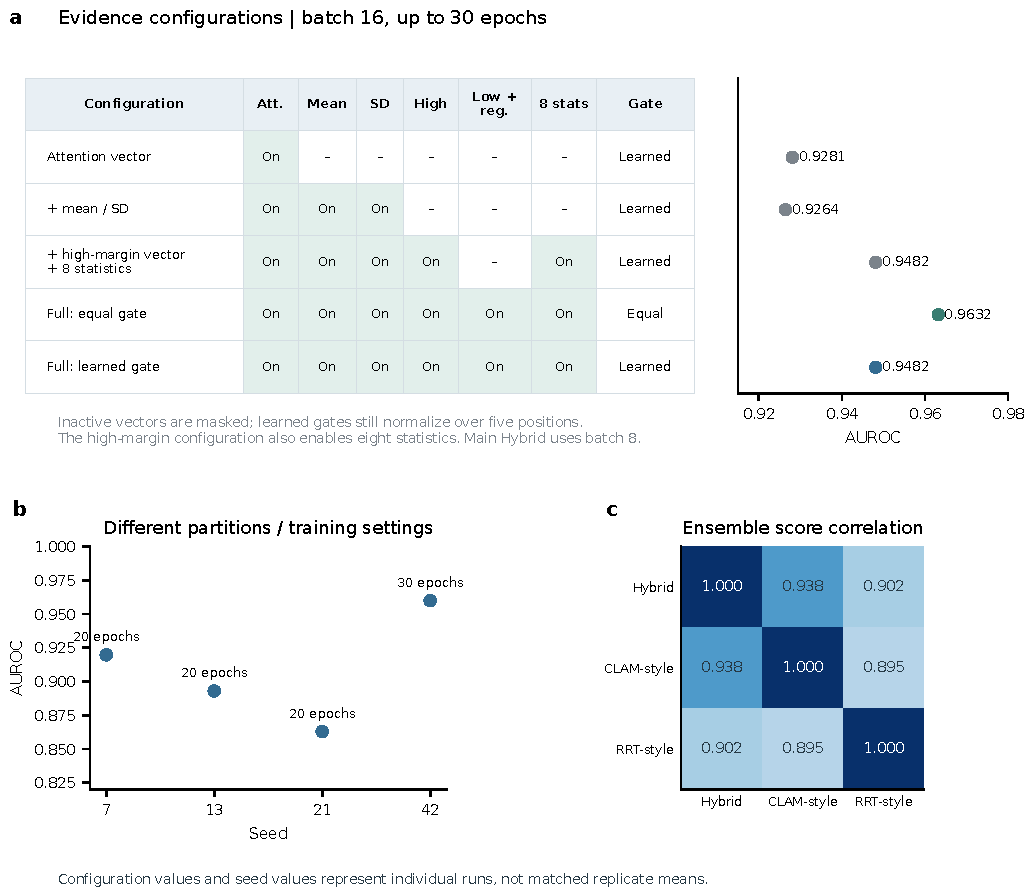
\includegraphics[width=\textwidth,height=.70\textheight,keepaspectratio]{figures/Supplementary_Figure_S3_historical_configurations.pdf}
\caption{\textbf{Historical compound configurations and run records}. \textbf{a,} Input activation matrix and individual configuration AUROCs. Enabling the high-margin vector also enables eight statistics; low-margin and regional vectors remain combined. Learned gates normalize over five positions even when input vectors are masked. These runs used batch size 16 and up to 30 epochs; patch-sampling randomness was not fully seed-controlled. \textbf{b,} Individual runs with different partitions and training settings, retained as historical records rather than matched stability replicates. \textbf{c,} Pearson correlations of ensemble-member scores on the same 49 slides. Every AUROC point represents one run; no replicate error bars are implied. Source data: configuration\_activation\_matrix.csv, ablation\_metrics.csv, seed\_runs.csv and ensemble\_member\_correlations.csv.}\label{fig:S3}
\end{figure}

\clearpage
\begin{table}[H]\centering
\caption{Sampling variability with the fixed Hybrid checkpoint}\label{tab:S10}
\small
\begin{tabular}{p{.47\textwidth}rr}
\toprule
Summary & Internal & External \\
\midrule
WSIs & 49 & 168 \\
Additional bags per WSI & 20 & 20 \\
Median within-slide score SD & 0.0120 & 0.0150 \\
Within-slide score SD, interquartile range & 0.0019--0.0475 & 0.0065--0.0318 \\
Maximum within-slide score SD & 0.1297 & 0.1241 \\
Median within-slide score range & 0.0474 & 0.0581 \\
WSIs crossing 0.5 across the 20 bags & 7/49 & 18/168 \\
SS WSIs crossing 0.5 & 4/26 & 3/16 \\
MALT WSIs crossing 0.5 & 3/23 & 15/152 \\
Per-draw AUROC, mean (SD) & 0.9599 (0.0056) & 0.8749 (0.0097) \\
Per-draw AUROC, range & 0.9498--0.9682 & 0.8549--0.8943 \\
20-bag mean-score AUROC (secondary) & 0.9632 & 0.8775 \\
20-bag mean-score sensitivity (secondary) & 95.65\% & 92.76\% \\
20-bag mean-score specificity (secondary) & 80.77\% & 75.00\% \\
\bottomrule
\end{tabular}
\par\medskip\raggedright\footnotesize Each technical repeat uses 512 sampled feature rows and the same frozen checkpoint. Standard deviations use the sample definition. Crossing means that at least one score is below 0.5 and at least one is at or above 0.5 among the 20 additional bags. AUROC spread across draws is not a confidence interval. Mean-score results are secondary summaries across all 20 bags and do not replace the archived single-bag results. Source data: sampling\_summary.csv, sampling\_per\_slide.csv and sampling\_per\_draw\_metrics.csv.
\end{table}
\clearpage
\begin{table}[H]\centering
\caption{External model comparisons on shared reference bags}\label{tab:S11}
\small
\begin{tabular}{p{.18\textwidth}p{.23\textwidth}p{.23\textwidth}p{.23\textwidth}}
\toprule
Model & AUROC (95\% interval) & Sensitivity (95\% interval) & Specificity (95\% interval) \\
\midrule
Hybrid & \textbf{0.8721} (0.7294--0.9737) & \textbf{93.42\%} (88.31--96.39) & \underline{68.75\%} (44.40--85.84) \\
ABMIL & \underline{0.7903} (0.6275--0.9268) & 42.76\% (35.17--50.71) & \textbf{81.25\%} (56.99--93.41) \\
CLAM-SB-style & 0.6591 (0.4568--0.8491) & 58.55\% (50.60--66.08) & 62.50\% (38.64--81.52) \\
RRTMIL-style & 0.7743 (0.6114--0.9100) & \underline{89.47\%} (83.59--93.42) & 50.00\% (28.00--72.00) \\
\bottomrule
\end{tabular}
\medskip
\begin{tabular}{p{.32\textwidth}rp{.27\textwidth}}
\toprule
Paired difference & AUROC difference & 95\% interval \\
\midrule
Hybrid minus ABMIL & 0.0818 & -0.0136 to 0.2011 \\
Hybrid minus CLAM-SB-style & 0.2130 & 0.0843 to 0.3528 \\
Hybrid minus RRTMIL-style & 0.0979 & 0.0415 to 0.1649 \\
\bottomrule
\end{tabular}
\par\medskip\raggedright\footnotesize Bold/underline mark the highest/second-highest point estimate in each metric column. All four original checkpoints were evaluated on identical per-slide reference bags from 168 WSIs (152 MALT and 16 SS). Sensitivity and specificity use threshold 0.5 and Wilson intervals. AUROC and paired-difference intervals in this new analysis use 10,000 label-stratified WSI bootstrap draws; the archived Hybrid intervals in main Table 3 use 2,000 draws. Differences are unadjusted descriptive comparisons of complete model implementations, not isolated aggregation mechanisms or confirmatory family-wise inference. Source data: reference\_model\_metrics.csv and external\_paired\_comparisons.csv.
\end{table}
\clearpage
\begin{table}[H]\centering
\caption{Archived segmentation-contour coverage of the eight displayed regions}\label{tab:S12}
\small Individual-case rows are omitted from this public repository copy.
\end{table}
\clearpage
\begin{table}[H]\centering
\caption{Descriptive Brier scores of archived predictions}\label{tab:S13}
\small
\begin{tabular}{llrl}
\toprule
Cohort & Model & WSIs & Brier score (95\% interval) \\
\midrule
Internal & Hybrid & 49 & 0.0895 (0.0429--0.1463) \\
Internal & ABMIL & 49 & 0.1056 (0.0396--0.1827) \\
Internal & CLAM-SB-style & 49 & 0.1002 (0.0561--0.1525) \\
Internal & RRTMIL-style & 49 & \underline{0.0894} (0.0341--0.1569) \\
Internal & Three-model ensemble & 49 & \textbf{0.0829} (0.0412--0.1330) \\
External & Hybrid & 168 & 0.0919 (0.0702--0.1156) \\
\bottomrule
\end{tabular}
\par\medskip\raggedright\footnotesize Bold/underline mark the lowest/second-lowest point estimate within each cohort; a lone estimate is unranked. Brier score is the mean squared difference between the uncalibrated sigmoid score and the binary label (MALT = 1). Intervals use 10,000 label-stratified WSI bootstrap resamples of fixed predictions. Seeds are recorded in the source table. No calibration function was fitted to either evaluation cohort. Brier score combines several aspects of probabilistic prediction and does not independently isolate calibration or establish clinical utility. Source data: brier\_descriptive.csv.
\end{table}
\clearpage
\begin{table}[H]\centering
\caption{Dimensions and parameter counts of the evaluated complete models}\label{tab:S14}
\small
\begin{tabular}{lrrrrr}
\toprule
Model & Head input & Attention width & Parameters & Epoch budget & Batch \\
\midrule
Hybrid & 256 & 256 & 1,521,672 & 30 & 8 \\
ABMIL & 1536 & 512 & 6,690,306 & 50 & 16 \\
CLAM-SB-style & 256 & 256 & 591,874 & 20 & 8 \\
RRTMIL-style & 256 & 256 & 1,711,874 & 20 & 4 \\
\bottomrule
\end{tabular}
\par\medskip\raggedright\footnotesize All models receive 1,536-dimensional UNI2-h features and use 512 sampled rows. Head input is the dimension passed from the slide encoder to the common classifier construction; its hidden width is 256. ABMIL retains 1,536-dimensional patch features with additional transformations before and after attention pooling, whereas Hybrid projects features to 256 dimensions and fuses five vectors with eight statistics. These differences, along with training budgets, prevent attribution to pooling alone. Parameter counts were obtained by strict loading of the archived checkpoints; they do not measure runtime, memory, or energy. Source data: model\_checkpoint\_inventory.csv and checkpoint\_tensor\_shapes.json.
\end{table}


\clearpage
\begin{table}[H]\centering
\caption{All predefined controlled training runs}\label{tab:S15}
\small
\begin{tabular}{lrrrrrr}
\toprule
Configuration & Seed & Epoch & \shortstack{Internal\\AUROC} & \shortstack{External\\AUROC} & \shortstack{External\\sensitivity} & \shortstack{External\\specificity} \\
\midrule
Matched attention & 17 & 13 & \textbf{0.9314} & \underline{0.8170} & \textbf{80.26\%} & 62.50\% \\
Matched attention & 29 & 18 & \underline{0.9331} & \underline{0.7500} & \textbf{61.18\%} & 62.50\% \\
Matched attention & 43 & 12 & 0.9398 & 0.6139 & \textbf{34.87\%} & 56.25\% \\
\addlinespace
Fixed scaling & 17 & 24 & 0.9231 & \textbf{0.8701} & 53.29\% & \textbf{87.50\%} \\
Fixed scaling & 29 & 18 & \textbf{0.9431} & 0.7442 & 56.58\% & \underline{68.75\%} \\
Fixed scaling & 43 & 25 & \textbf{0.9532} & \underline{0.6192} & 13.16\% & \underline{62.50\%} \\
\addlinespace
Learned gate & 17 & 29 & \underline{0.9298} & 0.7311 & \underline{60.53\%} & \underline{68.75\%} \\
Learned gate & 29 & 20 & \underline{0.9331} & \textbf{0.9350} & \underline{59.21\%} & \textbf{93.75\%} \\
Learned gate & 43 & 29 & \underline{0.9431} & \textbf{0.6238} & \underline{17.76\%} & \textbf{68.75\%} \\
\addlinespace
\bottomrule
\end{tabular}
\par\medskip\raggedright\footnotesize Bold/underline compare configurations within the same seed and metric column. Each run used the same original 144/49 training/evaluation partition, 30 epochs, batch size eight, learning rate $5\times10^{-5}$, weight decay $10^{-4}$, dropout 0.3 and positive-class loss weight $77/67$. Within each seed, configurations shared identical initial values for common tensors, training bags and minibatch order. The original internal and external reference bags were fixed. Epoch denotes the first epoch with the highest internal AUROC; external evaluation was performed after selection. All nine predefined runs are reported. Matched attention shares the 256-dimensional projection, attention block and classifier construction but omits the other vectors, statistics and fusion layer. Fixed scaling multiplies all five vectors by 0.2; learned gating also changes nonlinear capacity. Parameters: matched attention 658,178, fixed scaling 1,190,403, learned gate 1,521,672. Thus these are controlled configuration comparisons, not parameter-matched or isolated single-component tests. Across-seed summaries describe training variation in the same cohort and do not add independent WSIs. No three-seed significance test is used. Source data: run\_metrics.csv, configuration\_summary.csv and paired\_seed\_differences.csv.
\end{table}

\begin{figure}[H]\centering
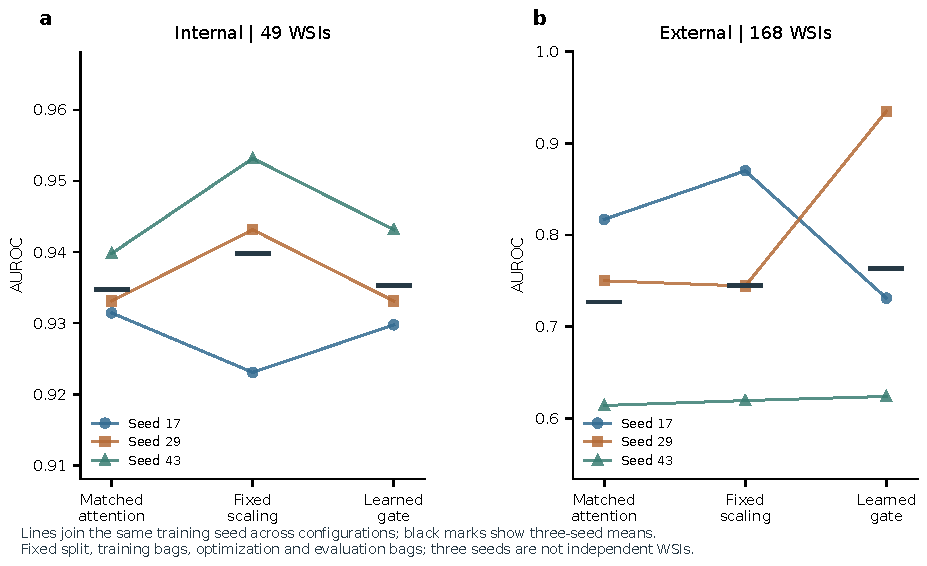
\includegraphics[width=\textwidth,height=.42\textheight,keepaspectratio]{figures/Supplementary_Figure_S4_controlled_training.pdf}
\caption{\textbf{Controlled configuration comparisons across three training seeds}. \textbf{a,b,} Internal and external AUROCs for every selected checkpoint from the nine predefined runs in Supplementary Table S15. Lines join the same seed across configurations and black horizontal marks denote three-seed means. Cohorts and evaluation inputs are unchanged across runs. Three seed values are descriptive training repeats rather than independent clinical observations; no confidence interval or inferential superiority claim is implied. Source data: run\_metrics.csv.}\label{fig:S4}
\end{figure}


% Controlled training results are synthesized in the main Results; S15/Fig. S4 retained.
